%!TEX ROOT=formularioFisica.tex

\section{Relatività}
La relatività rivoluziona il significato della Fisica moderna. Grazie ad Einstein ma non solo, si è
aperto un nuovo capitolo.

\subsection{Trasformazioni Galileiane}
Per comprendere la relatività, bisogna sapere che sistemi di riferimento si usavano in precedenza.
Essi erano ancora quelli di Galileo, del 1600. Si distinugono due tipi di sistemi di riferimento:
\textbf{inerziali} che soddisfano il principio di inerzia di Newton e \textbf{non inerziali} che
invece non lo soddisfano. Di sistemi inerziali assoluti, nella realtà, non ce ne sono.\\
Un sistema che si muove di Moto Rettilineo Uniforme rispetto ad un sistema inerziale. Questo sistema
è anch'esso inerziale. Andiamo a disegnare un sistema con un punto e il sistema che si è mosso.
\begin{center}
  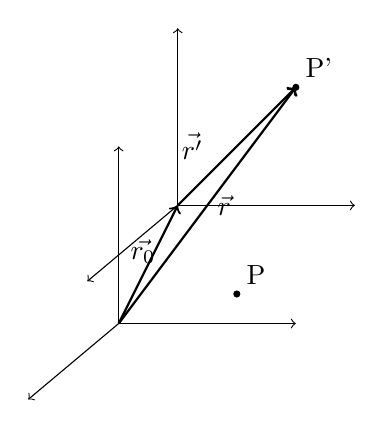
\begin{tikzpicture}[scale=0.75]
    \coordinate (O) at (0,0);
    \coordinate (O') at (1,2);
    \coordinate (P) at (2,0.5);
    \coordinate (P') at (3,4);

    \draw[->] (O) -- ++(0,3);
    \draw[->] (O) -- ++(3,0);
    \draw[->] (O) -- ++(220:2);

    \draw[->] (O') -- ++(0,3);
    \draw[->] (O') -- ++(3,0);
    \draw[->] (O') -- ++(220:2);
    
    \filldraw (P) circle (0.05);
    \filldraw (P') circle (0.05);

    \draw[->, thick] (O) -- (P')
      node[pos=0.5,right]{$\vec{r}$};
    \draw[->, thick] (O') -- (P')
      node[pos=0.3,above left]{$\vec{r'}$};
    \draw[->, thick] (O) -- (O')
      node[pos=0.8, below left]{$\vec{r_0}$};
    %\draw[->, thick] (P) -- (P')
    %  node[pos=0.5,right]{$\vec{v}$};

    \node[above right] at (P){P};
    \node[above right] at (P'){P'};
  \end{tikzpicture}
\end{center}
Con il calcolo vettoriale, possiamo sapere che $\vec{r} = \vec{r_0}+\vec{r'}$. In $t=0$, si ha che
$S \equiv S'$.\\
All'istante $t_1\,(t_1\neq0)$ si ha che
\begin{equation*}
  \vec{r_1} = \vec{r_1'} + \vec{v}t_1
\end{equation*}
All'istante $t_2\,(t_2\neq0)$ si ha che
\begin{equation*}
  \vec{r_2} = \vec{r_2'} + \vec{v}t_2
\end{equation*}
Trovando la differenza
\begin{equation*}
  \Delta \vec{r} = \Delta\vec{r'}+\vec{v}\Delta t
\end{equation*}
Dividendo per $t$
\begin{equation*}
  \frac{\Delta\vec{r}}{t}=\frac{\Delta\vec{r'}}{t}+\vec{v}
\end{equation*}
Che, considerando il rapporto spazio/tempo, si riscrive come
\begin{equation*}
  \vec{u} = \vec{u'}+\vec{v}
\end{equation*}
E questa è chiamata la \textbf{legge di composizione delle velocità}. Si ricordi che tutto ciò che
ha un apice (come $u'$) è relativo al sistema di riferimento $S'$.\\ [\baselineskip]
Imposto che $S'$ si muova di moto rettilineo uniforme sull'asse delle $x$ di $S$, le trasformazioni
galileiane sono così descritte
\begin{equation*}
  \begin{cases}
    x' = x-vt\\
    y'=y\\
    z'=z\\
    t'=t
  \end{cases}
\end{equation*}
L'ultima equazione è la più importante in questo caso. Essa infatti ci dice che \textbf{il tempo è
assoluto e non dipende dal sistema di riferimento}. 

\subsection{Esperimento di Michelson-Morley}
Nell'arco di venti e più anni, i due scienziati Michelson e Morley dimostrarono che la velocità della
luce non variava e che quindi il vento dell'etere, precedentemente teorizzato, non esisteva.
\subsubsection{Il vento dell'etere}
L'esperimento del vento dell'etere può essere riassunto così
\begin{center}
  \begin{tikzpicture}[square/.style={regular polygon,regular polygon sides=4}]
    \coordinate (A) at (0,0);
    \coordinate (B) at (3,0);
    \coordinate (C) at (0,3);

    \node at (A) [square,draw](A){A};
    \node at (B) [square,draw](B){B};
    \node at (C) [square,draw](C){C};

    \draw[|<->|] (A) -- (B)
      node[pos=0.5,below]{$L$};
    \draw[|<->|] (A) -- (C)
      node[pos=0.5,left]{$L$};

    \foreach\y in {2,1.5,1}{%
      \draw[->] (3,\y) -- ++(-2,0);
    }
  \end{tikzpicture}
\end{center}
Definendo $v_M$ la velocità del moto e $v_V$ la velocità del vento, si può immaginare un corpo che
segue la rotta A-B e un altro che segue quella A-C. LA teoria dice che i tempi impiegati dai due 
moti devono essere diversi se il vento dell'etere esistesse. Infatti si ha che
\begin{align*}
  t_\perp&<t_\|\\
  \intertext{Considerato che la velocità d'andata e di ritorno sono diverse, si devono sommare, si
  hanno che la somma è pari a $\frac{L}{v_M-v_V} + \frac{L}{v_M+v_V}$}
  \frac{2L}{\sqrt{v_M^2-v_V^2}}&<\frac{2v_M^2}{v_M^2-v_V^2}\\
  \frac{1}{v_M^2-v_V^2}&<\frac{v_M^2}{{(v_M-v_V)}^2}\\
  1&<\frac{v_M^2(v_M^2-v_V^2)}{(v_M^2-v_V^2)}\\
  1&<\frac{v_M^2}{v_M^2-v_V^2}\\
  v_M^2-v_V^2&<v_M^2
\end{align*}
e questo verifica la tesi.\\ [\baselineskip]
Essendo l'etere solidale al sole, le due velocità perpendicolari e parallele dovevano essere
diverse. Ma, attraverso un interferometro che hanno continuato a migliorare, hanno dimostrato che
$c$ è sempre costante, non è mai cambiata. Infatti la Terra ruotando doveva intercettare l'etere
in maniere diverse. Questo avrebbe dovuto causare nell'interferometro diverse configurazioni di
interferenza ma questo non si è mai visto.

\subsection{Principi fondamentali della relatività ristretta}
La prima forumulazione della relatività, è quella ristretta. Essa si fonda su due principi cardine:
\begin{enumerate}
  \item \textbf{Tutte le formule devono avere la stessa forma per ogni tipo di sistema inerziale}
  \item \textbf{La luce nel vuoto ha la stessa velocità per ogni sistema} 
\end{enumerate}
Questi due principi mettono in crisi la fisica classica. Infatti le recenti Equazioni di Maxwell non
erano invarianti secondo le trasformazioni galileiane.

\subsection{Simultaneità}
Einstein propone un esperimento mentale per illustrare che due eventi non sono simultanei se si tiene
conto dei principi della relatività. Infatti si immaginino due osservatori, $O$ su di una banchina
e $O'$ su di un treno in moto rettilineo uniforme rispetto a $O$ di velocità $\vec{v}$. Se 
$\vec{v}=\vec{0}$ ovviamente due qualsiasi eventi $E_1,E_2$ sarebbero simultanei per i due 
osservatori in quanto essi sarebbero nello stesso identico luogo.\\
Nel caso in cui però $\vec{v}\neq\vec{0}$, i due eventi non lo sono più. Infatti se esattamente 
quando $O\equiv O'$ si fanno partire due raggi luminosi a distanza uguale a destra e sinistra di $O$,
$O$ li vedrà arrivare nello stesso momento in quanto ha la stessa distanza da entrambi. $O'$ invece,
muovendosi, nel tempo che la luce impiega per raggiungerlo, avrà fatto un certo percorso e quindi 
vedrà i raggi in momenti diversi. $E_1$ ed $E_2$ non sono più simultanei per lui. Lo sarebbero se
$c=\infty$ ma è stato dimostrato che non è così.\\
Questo porta a due conseguenze
\begin{enumerate}
  \item \textbf{La dilatazione del tempo}
  \item \textbf{La contrazione della misura nella direzione del moto} 
\end{enumerate}

\subsection{Dilatazione del tempo}
Un orologio luminoso è composto da una sorgente luminosa posta ad un'estremità di una scatola di 
lunghezza $l$ e da uno specchio nell'altra. L'unità di tempo diventa quindi il tempo necessario alla
luce ad andare e tornare.\\
Si prendano due osservatori, $O$ su di una banchina e $O'$ su di un treno che si muove di velocità
$\vec{v}$ rispetto a $O$. Entrambi hanno un orologio luminoso. Si definisca $\Delta t'$ il tempo
misurato dall'orologio di $O$. Esso sarà pari a
\begin{equation*}
  \Delta t' = \frac{2l}{c}
\end{equation*}
Il tempo $\Delta t$ invece sarà diverso in quanto nel periodo in cui la luce raggiunge lo specchio,
il treno con l'ossevatore $O'$ si sarà spostato. Quindi si ha una situazione del genere
\begin{center}
  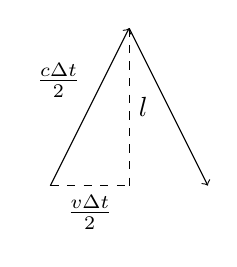
\begin{tikzpicture}
    \draw[->] (0,0) -- (1,2)
      node[pos=0.5,above left]{$\frac{c\Delta t}{2}$};
    \draw[->] (1,2) -- (2,0);
    \draw[dashed] (1,2) -- (1,0)
      node[pos=0.5,right]{$l$};
    \draw[dashed] (0,0) -- (1,0)
      node[pos=0.5,below]{$\frac{v\Delta t}{2}$};
  \end{tikzpicture}
\end{center}
Andando quindi a risolvere per $\Delta t$ abbiamo che
\begin{align*}
  {\left( \frac{c\Delta t}{2} \right)}^2&=l^2+{\left( \frac{v\Delta t}{2} \right)}^2\\
  \frac{c^2}{4}{(\Delta t)}^2&=l^2+\frac{v^2{(\Delta t)}^2}{4}\\
  (c^2-v^2){(\Delta t)}^2&={(2l)}^2\\
  (c^2-v^){(\Delta t)}^2 &= c^2{(\Delta t')}^2\\
  {(\Delta t)}^2&= \frac{c^2{(\Delta t')}^2}{c^2-v^2}\\
  \Delta t &= \frac{\Delta t'}{\sqrt{1-\frac{v^2}{c^2}}}
\end{align*}
Quindi abbiamo che $\Delta t\neq\Delta t'$. Anzi, per $v\ll c$ si ha che $\Delta t \to \Delta t'$.
$\Delta t'$ viene definito \textbf{tempo proprio}. Il termine
\begin{equation*}
  \gamma = \frac{1}{\sqrt{1-\frac{v^2}{c^2}}}
\end{equation*}
tornerà spesso fuori anche nelle trasformazioni di Lorentz, non è un caso si ritrovi anche lì.

\subsection{La velocità limite della luce}
Se si prende il fattore $\gamma$ e lo si studia, si capirà subito che non può esserci una velocità
maggiore $c$. Andando a fare un semplice studio di funzione si vede che
\begin{equation*}
  \mathcal{D}_\gamma = ]{-c},{c}[
\end{equation*}
ma poiché in fisica le velocità sono in genere positive, su può considerare solo $0 < v < c$.
Vediamo inoltre che $\gamma(-v) = \gamma(v)$. Andando a calcolare la derivata prima si trova
\begin{equation*}
  \der{\gamma(v)}{v} = \frac{v \left( 1-\frac{v^2}{c^2} \right)}{c^2\sqrt{1-\frac{v^2}{c^2}}}
\end{equation*}
Andando a studiare il segno vediamo che in $v=0$ ha un minimo. Andando a calcolare $\gamma(0)=1$.
Infine andando a fare il limite
\begin{equation*}
  \lim\limits_{v\to c^-} \gamma = +\infty 
\end{equation*}
si vede che $v=c$ è asintoto verticale e che quindi non è possibile superare la velocità della 
luce.\\
Questo, assieme al fatto che
\begin{equation*}
  \frac{\Delta t}{\Delta t'}=\gamma > 1
\end{equation*}
produce il fatto che $\Delta t > \Delta t'$ e che quindi si verifica una \textbf{dilatazione 
temporale}.

\subsection{Trasformazioni di Lorentz}
Le trasformazioni di Lorentz hanno la caratteristica di rendere invarianti le equazioni di Maxwell.
Presi due sistemi inerziali $S$ e $S'$ che si muovono sull'asse delle $x$ di moto rettilineo 
uniforme, le trasformazioni di Lorentz si scrivono come
\begin{equation*}
  \begin{cases}
    x'= \gamma(x-vt)\\
    y'=y\\
    z'=z\\
    t'=\gamma(t-\frac{v}{c^2}x)
  \end{cases}
\end{equation*}
La grande ed enorme novità sta proprio nell'ultima equazione, quella relativa al tempo. Sono due 
tempi diversi che dipendono dalla posizione e dalla velocità.\\
Presi due istanti $t_1',t_2'$ si ha che
\begin{equation*}
  \Delta t = t'_2\gamma -\cancel{\frac{vx}{c^2}\gamma}-t'_1\gamma+\cancel{\frac{vx}{c^2}\gamma}=
  \gamma\Delta t'
\end{equation*}
Che è esattamente lo stesso risultato ottenuto da Einstein nei suoi esperimenti mentali.

\subsection{Contrazione delle lunghezze}
Presi due sistemi di riferimento $S,S'$ che si muovono di moto rettilineo uniforme e un corpo di
lunghezza $L$ solidale a $S'$, i ue sistemi misureranno $L$ per $S$ e $L'$ per $S'$. Si ha
\begin{equation*}
  L'= x_B'-x_A'\quad L=x_B-x_A
\end{equation*}
Si ha inoltre che $x'=\gamma(x-vt)$. Calcolando allora
\begin{equation*}
  L' = x_B'-x_A'=\gamma(x_B-vt)-\gamma(x_A-vt)=\gamma(x_B-x_A)=\gamma L
\end{equation*}
Si ha quindi che
\begin{equation*}
  L = \frac{L'}{\gamma}
\end{equation*}
e che quindi le due lunghezze non sono misurate uguali dai due sistemi di riferimento.

\subsection{Piano di Minkowsky}
Minkowsky ha preso le trasformazioni di Lorentz e le ha guardate da un punto di vista puramente
matematico. Il suo piano è un piano simile
\begin{center}
  \begin{tikzpicture}
    \draw[->,thick] (-0.5,0) -- (3,0)
      node[pos=0.9,below]{$x$};
    \draw[->,thick] (0,-0.5) -- (0,3)
      node[pos=0.9,left]{$ct$};
  \end{tikzpicture}
\end{center}
Come mai $ct$ nell'asse delle $y$? Se un punto $P$ è definito da 4 variabili $P(x,y,z,t)$, non si
può avere tre unità di misura di lunghezza e una di tempo. Per uniformarle, si è moltiplicato il
tempo per una velocità (sempre costante), ottenendo una lunghezza.\\
Ma se un punto ha 4 coordinate, come può chiamarsi ``piano''? Sempre perché definiamo $y'=y$ e
$z'=z$. Quindi otteniamo che da $\mathbb{R}^4$ arriviamo a $\mathbb{R}^2$. Notiamo inoltre che il
piano, rispetto alla fisica classica, ha invertiti tempo e posizione.\\ [\baselineskip]
Andando a scrivere le equazioni di Lorentz con un termina $\beta = \frac{v}{c}$
\begin{equation*}
  \begin{cases}
    x' =\gamma(x-\beta ct)\\
    t'=\gamma\left(t-\beta\frac{x}{c}\right)
  \end{cases}
\end{equation*}
Per trovare l'asse verticale, poniamo $ct'=0$, $t'=0$ e che quindi $ct = \beta x$. Questo è il 
nuovo asse del piano di Minkowsky. Ponendo $x'=0$ si ha che $ct=\frac{x}{\beta}$ e che quindi 
abbiamo che la perpendicolare al primo-terzo quadrante è la retta che divide il piano. Praticamente
il piano ora diventa così
\begin{center}
  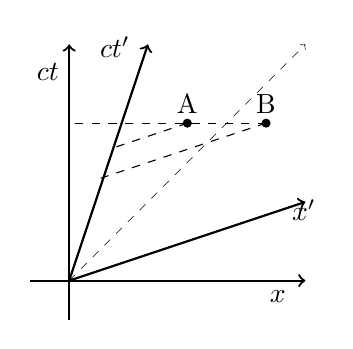
\begin{tikzpicture}
    \draw[->,thick] (-0.5,0) -- (3,0)
      node[pos=0.9,below]{$x$};
    \draw[->,thick] (0,-0.5) -- (0,3)
      node[pos=0.9,left]{$ct$};
    \draw[->,thick] (0,0) -- (1,3)
      node[pos=0.9,above left]{$ct'$};
    \draw[->,thick] (0,0) -- (3,1)
      node[pos=0.9,right]{$x'$};
    \draw[->,dashed,very thin] (0,0) -- (3,3);
    \filldraw (2.5,2) circle (0.05)
      node[above]{B};
    \filldraw (1.5,2) circle (0.05)
      node[above]{A};
    \draw[dashed] (2.5,2) -- (0,2);
    \draw[dashed] (2.5,2) -- (0.4,1.3);
    \draw[dashed] (1.5,2) -- (0.6,1.7);
  \end{tikzpicture}
\end{center}
Da questo vediamo una cosa che è fondamentale. $t_A=t_B$ ma $t'_A\neq t'_B$.

\subsection{Invariante spazio-temporale}
Minkowsky aveva trovato un'invariante nelle equazioni di Lorentz. Essa era $\sigma$. Infatti è
definita come
\begin{equation*}
  {(\Delta\sigma)}^2={(c\Delta t)}^2-{(\Delta S)}^2
\end{equation*}
Dove $\Delta S$ è la differenza della variazione di tutte le coordinate. Si ha quindi che
\begin{align*}
  \Delta x' &= \gamma(\Delta x-v\Delta t)\\
  \Delta y' &= \Delta y\\
  \Delta z' &= \Delta z\\
  \Delta t' &= \gamma \left( \Delta t-\frac{v}{c^2}\Delta x \right)
\end{align*}
Sostituendo ora, sono solo conti
\begin{align*}
  {(\Delta\sigma')}^2 &= {(c\Delta t')}^2-{(\Delta x')}^2-{(\Delta y')}^2-{(\Delta z')}^2\\
                      &= {\left(c\left(\gamma \left( \Delta t-\frac{v}{c^2}\Delta x \right)\right)
                      \right)}^2-
  {\left( \gamma \left( \Delta x-v\Delta t \right) \right)}^2-{(\Delta y)}^2-{(\Delta z)}^2\\
  &= c^2\gamma^2 \left[ {(\Delta t)}^2+\frac{v^2}{c^2}{(\Delta x)}^2-\frac{2v}{c^4}{(\Delta x)}^2 -
  \frac{2v}{c^2}\Delta x\Delta t\right]-\\
  &\gamma^2({(\Delta x)}^2+v^2{(\Delta t)}^2-2\Delta x\Delta t)-{(\Delta y)}^2-{(\Delta z)}^2\\
  &=\gamma^2 \left[ c^2{(\Delta t)}^2+\frac{v^2}{c^4}{(\Delta x)}^2-v{(\Delta t)}^2 \right]-
  {(\Delta y)}^2-{(\Delta z)}^2\\
  &=\gamma^2 \left[ (c^2-v^2){(\Delta t)}^2-\left( 1-\frac{v^2}{c^2}
  {(\Delta x)}^2 \right){(\Delta x)}^2 \right]-{(\Delta y)}^2-
  {(\Delta z)}^2\\
  &=\frac{c^2}{c^2v^2}\left[ (c^2-v^2){(\Delta t)}^2-\left( \frac{c^2-v^2}{v^2}
  \right){(\Delta x)}^2 \right]-{(\Delta y)}^2-{(\Delta z)}^2\\
  &=c^2{(\Delta t)}^2-{(\Delta x)}^2-{(\Delta y)}^-{(\Delta z)}^2\\
  &={(\Delta\sigma)}^2
\end{align*}
